\documentclass[handout]{beamer}

\usetheme[progressbar=frametitle]{metropolis}
\metroset{block=fill}

\subtitle{NTIN071 Automata and Grammars}
\author{Jakub Bulín (KTIML MFF UK)}

\date{Spring 2025\\ 
    \vspace{1in} 
    \begin{flushleft}
        \it \footnotesize * Adapted from the Czech-lecture slides by Marta Vomlelová with gratitude. The translation, some modifications, and all errors are mine.
    \end{flushleft}
}

%% packages

\usepackage{amsmath}
\usepackage{amssymb}
\usepackage{amsthm}
\usepackage{cancel}
\usepackage{color}
\usepackage{colortbl}
\usepackage{forest}
\usepackage[utf8x]{inputenc}
\usepackage{multicol}
\usepackage{multirow}

%% colors
\definecolor{Gray}{gray}{0.9}

%% TikZ
\usepackage{tikz}
    \usetikzlibrary{
        automata,
        arrows,
        backgrounds,
        decorations.pathmorphing,
        fit,
        positioning,
        shapes,
        shapes.geometric,
        tikzmark
    } 
    \tikzset{>=stealth',shorten >=1pt,auto,node distance=2cm}
    \tikzset{initial text={}}
    \tikzset{elliptic state/.style={draw,ellipse}}

%% amsthm
\theoremstyle{plain}
    \newtheorem*{algorithm}{Algorithm}    
    \newtheorem*{observation}{Observation}
    \newtheorem*{proposition}{Proposition}

\theoremstyle{remark}
    \newtheorem*{exercise}{Exercise}
    \newtheorem*{remark}{Remark}

%% macros
\DeclareMathOperator{\RegE}{RegE}
\DeclareMathOperator{\RL}{RL}

% Just for Lecture 2
\newcommand{\x}{$\times$}
\newcommand{\nx}{\ }



\title{Lecture 11 -- Turing Machines and grammars, Linear bounded automata and context-sensitive grammars, Intro to computability theory}


\begin{document}


\frame{\titlepage}


\begin{frame}{Recap of Lecture 10}
	
    \begin{itemize}        
        \item Turing machine: two-way infinite tape, read, write, move head
        \item Accept iff in a final state; configurations
        \item TMs with output, computing a function
        \item Recursively enumerable vs. recursive languages (always halt).
        \item Construction tricks: 
        \begin{itemize}
            \item storage in state
            \item multiple tracks (on a single tape)
        \end{itemize}
        \item Variants of TMs: 
        \begin{itemize}
            \item multi-tape (independent heads),
            \item nondeterministic (accept iff some choices lead to final state)
        \end{itemize}  
    \end{itemize}
	
\end{frame}


\section{3.3 Turing Machines and grammars}


\begin{frame}{Chomsky hierarchy: type 0}

    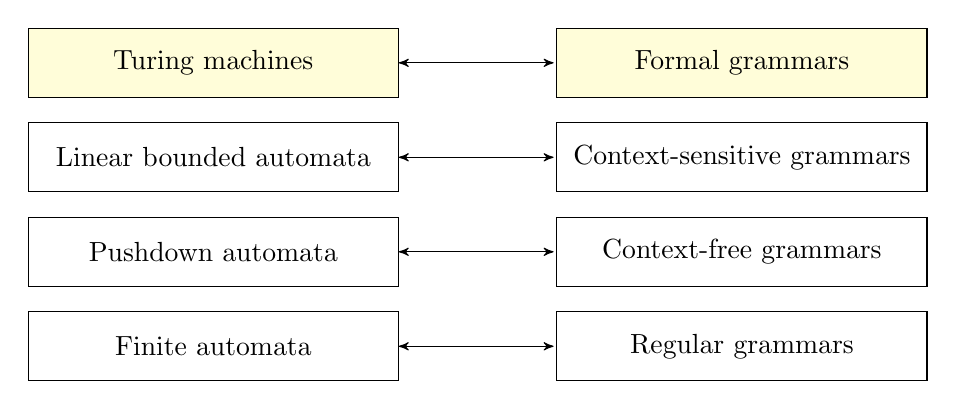
\begin{tikzpicture}[node distance=1.2cm]
        \node[state,rectangle, minimum width =4.7cm][align=center] (fa)      {\alert{Finite automata}};
        \node[state,rectangle, minimum width =4.7cm] (pda) [above of=fa]  {Pushdown automata};
        \node[state,rectangle, minimum width =4.7cm] (la) [above of=pda]  {Linear bounded automata};
        \node[fill=yellow!15!white,state,rectangle, minimum width =4.7cm][align=center] (ts) [above of=la]  {\alert{Turing machines}};
        \node[state,rectangle, minimum width =4.7cm] (rg) [right=2cm of fa]  {Regular grammars};
        \node[state,rectangle, minimum width =4.7cm]  (cfg) [right=2cm of pda]  {\alert{Context-free grammars}};
        \node[state,rectangle, minimum width =4.7cm][align=center]  (cg) [above of=cfg]  {Context-sensitive grammars};
        \node[fill=yellow!15!white,state,rectangle, minimum width =4.7cm] (g0) [above of=cg]  {Formal grammars};
        \path[<->] 
            (fa)  edge node {} (rg)
            (pda)  edge node {} (cfg)
            (la)  edge node {} (cg)
            (ts)  edge node {} (g0)
        ;
    \end{tikzpicture}

    \bigskip

    \begin{theorem}
        A language is recursively enumerable, if and only if it is generated by a Type 0 grammar.
    \end{theorem}
    

\end{frame}


\begin{frame}{Turing machine to grammar}
    
    \begin{itemize}
        \item First generate the relevant portion of the tape and a copy of the input word (nonterminal $\underline{X}$ for each $x\in\Gamma$, in 
        reverse)
        \item Why? TM can rewrite $w$, $G$ must generate it, cannot modify
        \item We have \alert{$wB^n\underline{W}^RQ_0B^m$}, where $B^n$, $B^m$ is sufficient free space        
        \item Then simulate moves (essentially reverse configs+free space)
        \item In a final state erase the simulated tape, keep only $w$
    \end{itemize}
    {\small
    $G=(\{S,C,D,E\}\cup \{\underline{X}\}_{x\in \Gamma}\cup \{Q_i\}_{q_i \in Q},\Sigma,\mathcal P,S)$ where $\mathcal P$ is:
    
    \begin{tabular}{lll}
        (1) 
        & $S\rightarrow DQ_0E$ 
        & simulation starts in initial state 
        \\

        & $D\rightarrow xD\underline{X}\mid E$ 
        & generate input word, reverse copy for simulation
        \\

        & $E\rightarrow BE\mid\epsilon$ 
        & generate sufficient free space for simulation
        \\        
        (2)
        & $\underline{X}P \rightarrow Q\underline{X'} $ 
        & for all $\delta(p,x)=(q,x',R)$ [direction reversed!]
        \\

        & $\underline{X}P \underline{Y}\rightarrow \underline{X'} \underline{Y}Q$ 
        & for all $\delta(p,x)=(q,x',L)$
        \\
        (3) 
        & $P\rightarrow C$ 
        & for all $p\in F$
        \\

        & $C \underline{X}\rightarrow C$,$\underline{X} C\rightarrow C$ 
        & clean the tape
        \\
        
        & $C\rightarrow \epsilon$ 
        & finish, generated $w$
    \end{tabular}
    }

\end{frame}


\begin{frame}{Example: $L=\{a^{2n}| n\geq 0\}$}

    $M=(\{q_0,q_1,q_2,q_F\},\{a\},\{a\},\delta,q_0,B,\{q_F\})$ where 
    \begin{align*}
        \delta(q_0,a)&=( q_1,a,R),\\
        \delta(q_1,a)&=(q_0,a,R), \\
        \delta(q_0,B)&=(q_F,B,L)
    \end{align*}
        
    $G=(\{S,C,D,E,Q_0,Q_1,Q_F,\underline{a}\},\{a\},S,\mathcal P_1\cup\mathcal P_2\cup\mathcal P_3)$ \\

    \begin{multicols}{3}
        
        \textbf{Initialize:} $\mathcal P_1$\\
        $S\rightarrow DQ_0E$\\
        $D\rightarrow aD\underline{a}\mid E$\\        
        $E\rightarrow BE\mid\epsilon$

        \newcolumn

        \textbf{Simulate:} $\mathcal P_2$\\
        $\underline{a}Q_0\rightarrow Q_1\underline{a}$\\
        $\underline{a}Q_1\rightarrow Q_0\underline{a}$\\
        $BQ_0\underline{a}\rightarrow B\underline{a}Q_F$
        
        \newcolumn

        \textbf{Cleanup:} $\mathcal P_3$\\
        $Q_F\rightarrow C$\\
        $C\underline{a}\rightarrow C$\\
        $\underline{a}C\rightarrow C$\\
        $BC\rightarrow C$\\
        $C\rightarrow\epsilon$
        
    \end{multicols}
    
    \vspace{-12pt}

    For $w=aa$: initialize \alert{$aaB\underline{a}\underline{a}Q_0$},
     simulate \alert{$aaB\underline{a}Q_F\underline{a}$}, cleanup: \alert{$aa$}

\end{frame}


\begin{frame}{Proof}

    
% Why $L(T)=L(G)$?
% \begin{itemize}
% 	\item $w\in L(T)$
	
% 	\begin{itemize}
% 		\item there exists a finite accepting sequence of steps $T$ (finite space)
% \item the grammar generates sufficient space
% \item it simulates the moves and cleans non--input symbols
% 	\end{itemize}
% \item $w\in L(G)$
% \begin{itemize}
% 	\item the rules need not be in our order
% 	\item we may sort the derivation steps to ordering (1),(2),(3)
% 	\item underlined symbols were erased, therefore accepting state must have been generated
% 	\end{itemize}
%     \hfill\qedsymbol
% \end{itemize}

\end{frame}


\begin{frame}{Grammar to Turing machine}

    

\end{frame}



\section{3.4 Linear bounded automata and context-sensitive grammars}


\section{\sc Chapter 4: Intro to computability theory}





\end{document}


% \section*{From a grammar to a TM}
% \begin{theorem}
% Any Type 0 language is recursively enumerable.
% \end{theorem}
% \begin{proof} Idea: the TM generates sequentially all possible derivations
% \begin{itemize}
% 	\item we code $S\Rightarrow \omega_1\Rightarrow \ldots \Rightarrow  \omega_n=w$ as a word $\#S\#\omega_1\#\ldots \#w\#$
% 	\item we can construct a TM accepting words $\#\alpha\#\beta\#$ where $\alpha\Rightarrow\beta$
% 	\item we can construct a TM accepting words $\#\omega_1\#\ldots\#\omega_k\#$ where $\omega_1\Rightarrow^*\omega_k$
%     \item we can construct a TM generating sequentially all possible words.
% \end{itemize}

% \tikzstyle{startstop} = [rectangle, rounded corners, minimum width=2cm, minimum height=1cm,text centered, draw=black]
% \tikzstyle{io} = [trapezium, trapezium left angle=70, trapezium right angle=110, minimum width=3cm, minimum height=1cm, text centered, draw=black, fill=blue!30]
% \tikzstyle{process} = [rectangle, minimum width=3cm, minimum height=1cm, text centered, draw=black]
% \tikzstyle{decision} = [diamond,  aspect=2, text width=2cm, minimum height=1cm, text centered, draw=black]
% %\tikzstyle{process} = [rectangle, minimum width=3cm, minimum height=1cm, text centered, text width=3cm, draw=black, fill=orange!30]
% \tikzstyle{arrow} = [thick,->,>=stealth]

% \begin{tikzpicture}[node distance=4.5cm]
% %\draw[help lines,use as bounding box] (-1.5,-1.5) grid (6,0.8);
% \useasboundingbox (-1.5,-1.5) grid (6,0.8);
%     \scope[transform canvas={scale=1}]
% \node (start) [process] {generate (next) word};
% \node (dec1) [decision, right of=start] {word represents\\a derivation};
% \node (dec2) [decision, right of=dec1] {derivation\\ends with $w$};
% \node (s0) [draw=none, below=1.5cm of start] {};
% \node (c0) [draw=none, below=1cm of dec1] {};
% \node (d0) [draw=none, below=1cm of dec2] {};
% \node (d2) [draw=none, right=1cm of dec2] {};
% %%\node (pro2b) [process, right of=dec1, xshift=2cm] {Process 2b};
% \draw [arrow] (dec1) -- node {yes} (dec2);
% \draw [arrow] (dec2) -- node {yes} (d2);
% \draw [arrow] (dec1) -- node {no} (c0);
% \draw [arrow] (dec2) -- node {no} (d0);
% \draw [arrow] (s0) -- node {} (start);
% \draw [arrow] (start) -- node {} (dec1);
% %\draw [arrow] (dec2) |- (dec1);
% \path[-]
% 				(d0)  edge node {} (c0)
% 				(s0)  edge node {} (c0)
% ;
% \endscope
% \end{tikzpicture}
% \end{proof}